\documentclass[11pt]{article}
\usepackage{geometry}
\usepackage{amsmath}
\usepackage{amssymb}
\usepackage{enumitem}
\usepackage{fancyhdr}
\usepackage{palatino}
\usepackage{graphicx}
\pagestyle{fancy}

\lhead{MTH 201 (Calculus)}
\chead{Global Optimization}
\rhead{2018-10-29}

\begin{document}

\begin{center}
    \Large{Activities for 2018-10-29}
\end{center}


\subsection*{1. Review}
Here's the graph of a function, which is defined only on the closed interval $[-8,8]$. 
\begin{center}
    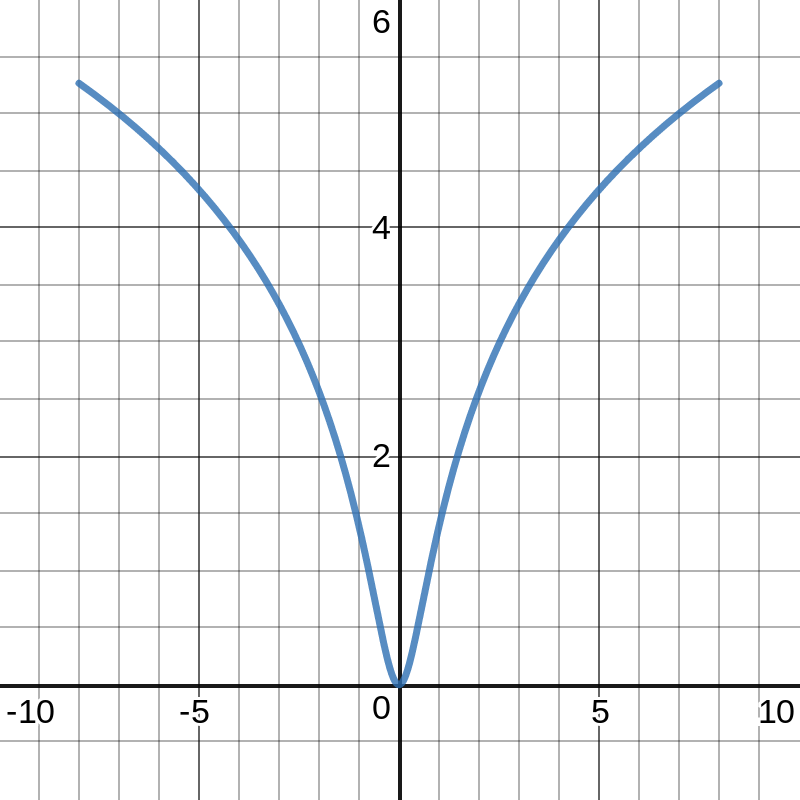
\includegraphics[width=3in]{34-review.png}
\end{center}
Using only this graph, list or label: 
\begin{itemize}
    \item The intervals where the function is increasing, and the intervals where the function is decreasing
    \item The intervals where the function is concave up and the intervals where the function is concave down
    \item The critical numbers of the function
    \item The local minima and local maxima of the function
    \item The absolute minima and absolute maxima of the function
    \item The inflection points of the function
\end{itemize}
The Desmos graph is here, if you want to play with it: 
\begin{center}
    https://www.desmos.com/calculator/e8xyd7k2ye 
\end{center}


\subsection*{2. Basic practice on global optimization}

Below are three functions. Each function comes with a closed interval, and you are to assume that the function is defined only on this interval. You may assume that the function is also continuous on that interval. Your group will be assigned one of these functions. Use the process from the reading of Section 3.3 to find the absolute minmum and absolute maximum values of the function on this interval. State both the values (that is, the output) and the $x$-coordinates of where those values happen. 

\begin{enumerate}
    \item $h(x) = xe^{-x}$, $[0,3]$
    \item $p(t) = \sin(t) + \cos(t)$, $[-\pi/2, \pi/2]$
    \item $j(s) = s \ln (s)$, $[1/4, 2]$
\end{enumerate}

\subsection*{3. Looking ahead to applied optimization}

A homeowner is interested in building a vegetable garden against one side of her house. The garden will be in a rectangular shape with one side of the rectangle being the house itself; the other three sides will use fencing material to keep animals out. Here's a picture: 

\begin{center}
    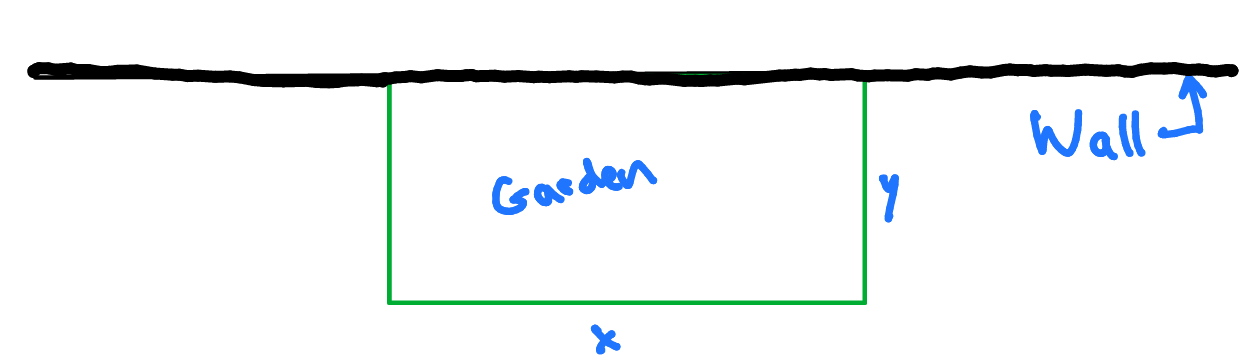
\includegraphics[width=5in]{optimization.png}}
\end{center}

The homeowner has 40 feet of fencing to use, and she would like to build the garden with the largest possible area out of that fencing. What should be the length and width of the garden that would create the largest possible area? 

\begin{enumerate}
    \item First play with the problem a little. One possible way to make the fence and use all 40 feet of fencing is to make $x = 20$ and $y = 10$. What's the area in that case? Now, what if $x = 10$ and $y = 15$? Try one more possible arrangement and find the area. This will show you that 40 feet of fencing can be arranged in different ways to yield different areas. 
    \item Write an expression (not an equation, just a mathematical expression) that gives the total amount of fencing used for any $x$ and any $y$. What does this expression have to equal in this situation?
    \item Now write an expression that gives the total \emph{area} enclosed by the garden. 
    \item Since we want to find the maximum possible value of area, we might try using our techniques from today's section. Can we take the derivative of the area expression? Why or why not? 
    \item Use the equation for total fencing length to make a substitution into the area formula, that will reduce it to one variable. 
    \item You now should have area as a function of a single variable. Notice that this variable cannot be negative due to physical reality; so its lowest possible value is 0. Is there an upper limit on what the variable can be? (Spoiler: The answer is ``yes''; what is that upper limit?)
    \item Now the area function is  continuous and defined on a closed interval. Find out the values of $x$ and $y$ that maximize the area, and state what that maximum value is. 
\end{enumerate}

\end{document}